\chapter{Benutzertests- und Interviews (Flelix)}
\label{chap:flinterviews}

	Es wurden drei Interviews mit Personen durchgeführt, welche die App bewerten sollen. Den Probanden wurde dabei jeweils nur erklärt, was der Nutzen einer Messung und Simulation von \textit{MEGA m.a.x.} und wofür die App dienen soll, alles weitere mussten sich die Personen selbst erarbeiten. Damit sollte getestet werden, ob die App intuitiv benutzbar und gut zu bedienen sind. Die Probanden sollten die App jeweils an Hand dieser vier Punkte bewerten:
	\begin{itemize}
		\item Wie ist der erste Eindruck?
		\item Was ist positiv aufgefallen?
		\item Was ist negativ aufgefallen?
		\item Ist die App intuitiv bedienbar?
	\end{itemize}

	Nach der Beantwortung dieser Fragen wird jeweils noch beschrieben, welche Anpassungen auf Grund des Feedbacks des jeweiligen Interviews durchgeführt wurden.

	\section{Benutzertest- und Interview 1}
	\label{sec:flinterview1}
	
	\paragraph{Wie ist der erste Eindruck?}
	
		Mein erster Eindruck der App ist sehr positiv. Die Corporate Indentity ist konsequent umgesetzt worden und die Farben sind untereinander sehr stimmig. Des Weiteren ist die Geschwindigkeit der App sehr hoch, sodass man nie lang warten muss. Sogar die Simulation von Eingabewerten geht sehr schnell, obwohl ich mir vorstellen kann, dass sehr komplexe Berechnungen dahinterstehen.
	
	\paragraph{Was ist positiv aufgefallen?}
		
		Wie bereits erwähnt, ist mir die hohe Geschwindigkeit der App aufgefallen. Auch die übersichtliche Darstellung, sowohl der veränderbaren Werte, als auch der simulierten Werte, sorgt meiner Meinung nach dafür, dass die App in sich sehr aufgeräumt wirkt.
	
	\paragraph{Was ist negativ aufgefallen?}
	
		Ein Punkt, der mir nicht so gut gefallen hat ist, dass das Textfeld für den Kommentar nur eine Zeile hat. Drückt man innerhalb dieses Textfeldes auf ``Enter'', wo wird dieses um eine Zeile länger. Ich finde dies sehr unintuitiv, weil sonst die Gefahr besteht, dass der Benutzer denkt, dass dort nur einzeilige Kommentare möglich sind.
	
	\paragraph{Ist die App intuitiv bedienbar?}
	
		Nach der Einführung in \textit{MEGA m.a.x.} und eine Erläuterung, wofür diese App dienen soll, konnte ich direkt loslegen und Profile anlegen sowie Simulationen durchführen. Es war keine weitere Anleitung notwendig, was sehr für die Intuitivität spricht. 
	
	\begin{figure}[H]
		\centering
		\begin{subfigure}[b]{0.45\textwidth}
			\centering
			
\includegraphics[width=1\textwidth]{../include/images/usertests/commentTextfield/before}
		\end{subfigure}
		\hfill
		\begin{subfigure}[b]{0.45\textwidth}
			
\includegraphics[width=1\textwidth]{../include/images/usertests/commentTextfield/after}
		\end{subfigure}
		\label{img:commentTextfield}
		\caption{Links: Kommentarfeld vor dem Interview, rechts nach dem Interview}
	\end{figure}

	Nach Durchführung des Interviews wurde das Kommentarfeld so angepasst, dass es etwas größer ist, um Verwirrung zu vermeiden. Dies ist in \cref{img:commentTextfield} zu sehen. Um diesen Effekt zu erreichen, wurde die Eigenschaft |minLines| des |TextField|s auf den Wert 4 gesetzt, vorher war dieser nicht gesetzt.
	
	\section{Benutzertest- und Interview 2}
	\label{sec:flinterview2}
	
	\paragraph{Wie ist der erste Eindruck?}
	
		Die App wirkt auf den ersten Blick sehr strukturiert und leicht zu bedienen. Wäre ich ein potentieller Kunde von Scheibner, würde es mir auf jeden Fall Spaß machen, mit dieser App zu arbeiten. Nach einiger Zeit habe ich die bildliche Darstellung der Simulationsergebnisse in Form von Diagrammen entdeckt, welche die Ergebnisse sehr anschaulich darstellen.
	
	\paragraph{Was ist positiv aufgefallen?}
		
		Mir haben die Einstellungsmöglichkeiten sehr gut gefallen. Es ist beispielsweise für einen Benutzer immer angenehmer, wenn die App automatisch in seiner Landessprache gestaltet ist und nicht in einer ``Standardsprache'' wie englisch. Weiterhin bietet die Einstellung, die Eingabe der veränderbaren Werte wahlweise durch Textfelder oder per Slider vorzunehmen, sehr viel Komfort. Will man einen sehr genauen Wert eingeben, so ist die Eingabe per Textfeld von Vorteil, soll nur eine ungefähre Simulation durchgeführt werden, so eignen sich die Slider besser, weil die Werte so schnell verändert werden können.\\
		Ein weiterer Punkt, der mir sehr positiv aufgefallen ist, dass mehrere Fahrzeuge, sprich Profile in der App angelegt und verwaltet werden können. Dies bietet insbesondere Besitzern von mehreren Motorrädern die Möglichkeit, all ihre Fahrzeuge in einer App zu simulieren.
	
	\paragraph{Was ist negativ aufgefallen?}
	
		Was mir nicht gut gefallen hat, ist die Tatsache, dass die Einstellungen auf der Einstellungsseite nicht sehr gut zu erkennen waren. Das lag daran, dass die Texte schwarz und der Hintergrund ein sehr dunkles grau sind.	
	
	\paragraph{Ist die App intuitiv bedienbar?}
		
		Da ich keinerlei weitere Anleitung benötigt habe, ist die App aus meiner Sicht intuitiv bedienbar. Für die Anwender, die vorher immer in eine Werkstatt vor Ort gehen mussten, um eine neue Simulation auszuführen, wird sie sicherlich einen hohen Mehrwert haben. Für die Werkstätten hat dies auch den Vorteil, dass sich die Mitarbeiter nicht mehr mit der stupiden Arbeit der Simulation befassen müssen: Es reicht dann, die Messung durchzuführen, dem Kunden die ID der Messung mitzuteilen und dieser kann die Simulation bequem selbst zu Hause durchführen. Schließlich kann er mit seinen angepassten und fertig simulierten Werten zurück zur Werkstatt kommen, um sein Motorrad entsprechende umzurüsten.

	\begin{figure}[H]
		\centering
		\begin{subfigure}[b]{0.45\textwidth}
			\centering
			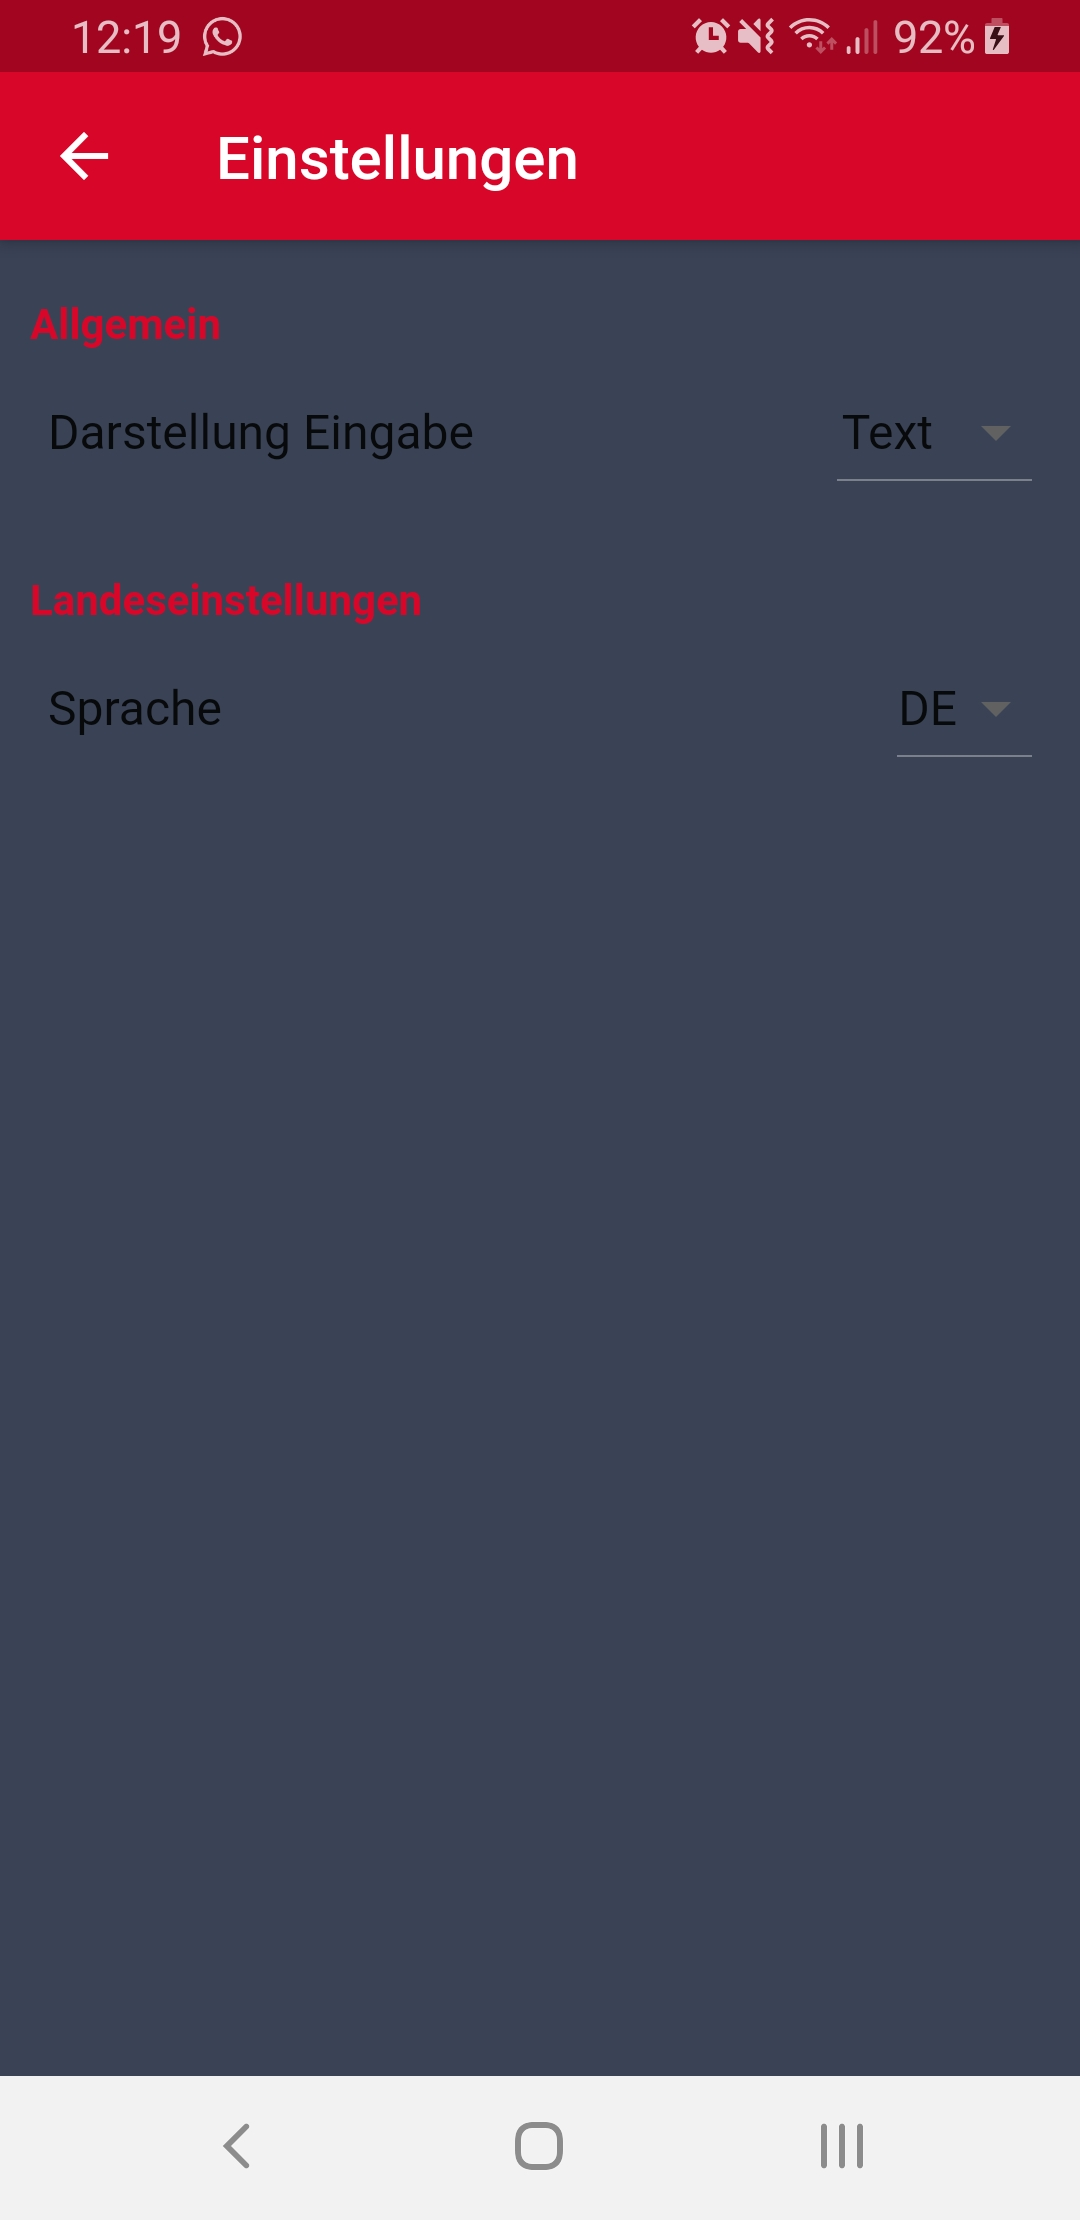
\includegraphics[width=1\textwidth]{../include/images/usertests/colorSettings/before}
		\end{subfigure}
		\hfill
		\begin{subfigure}[b]{0.45\textwidth}
			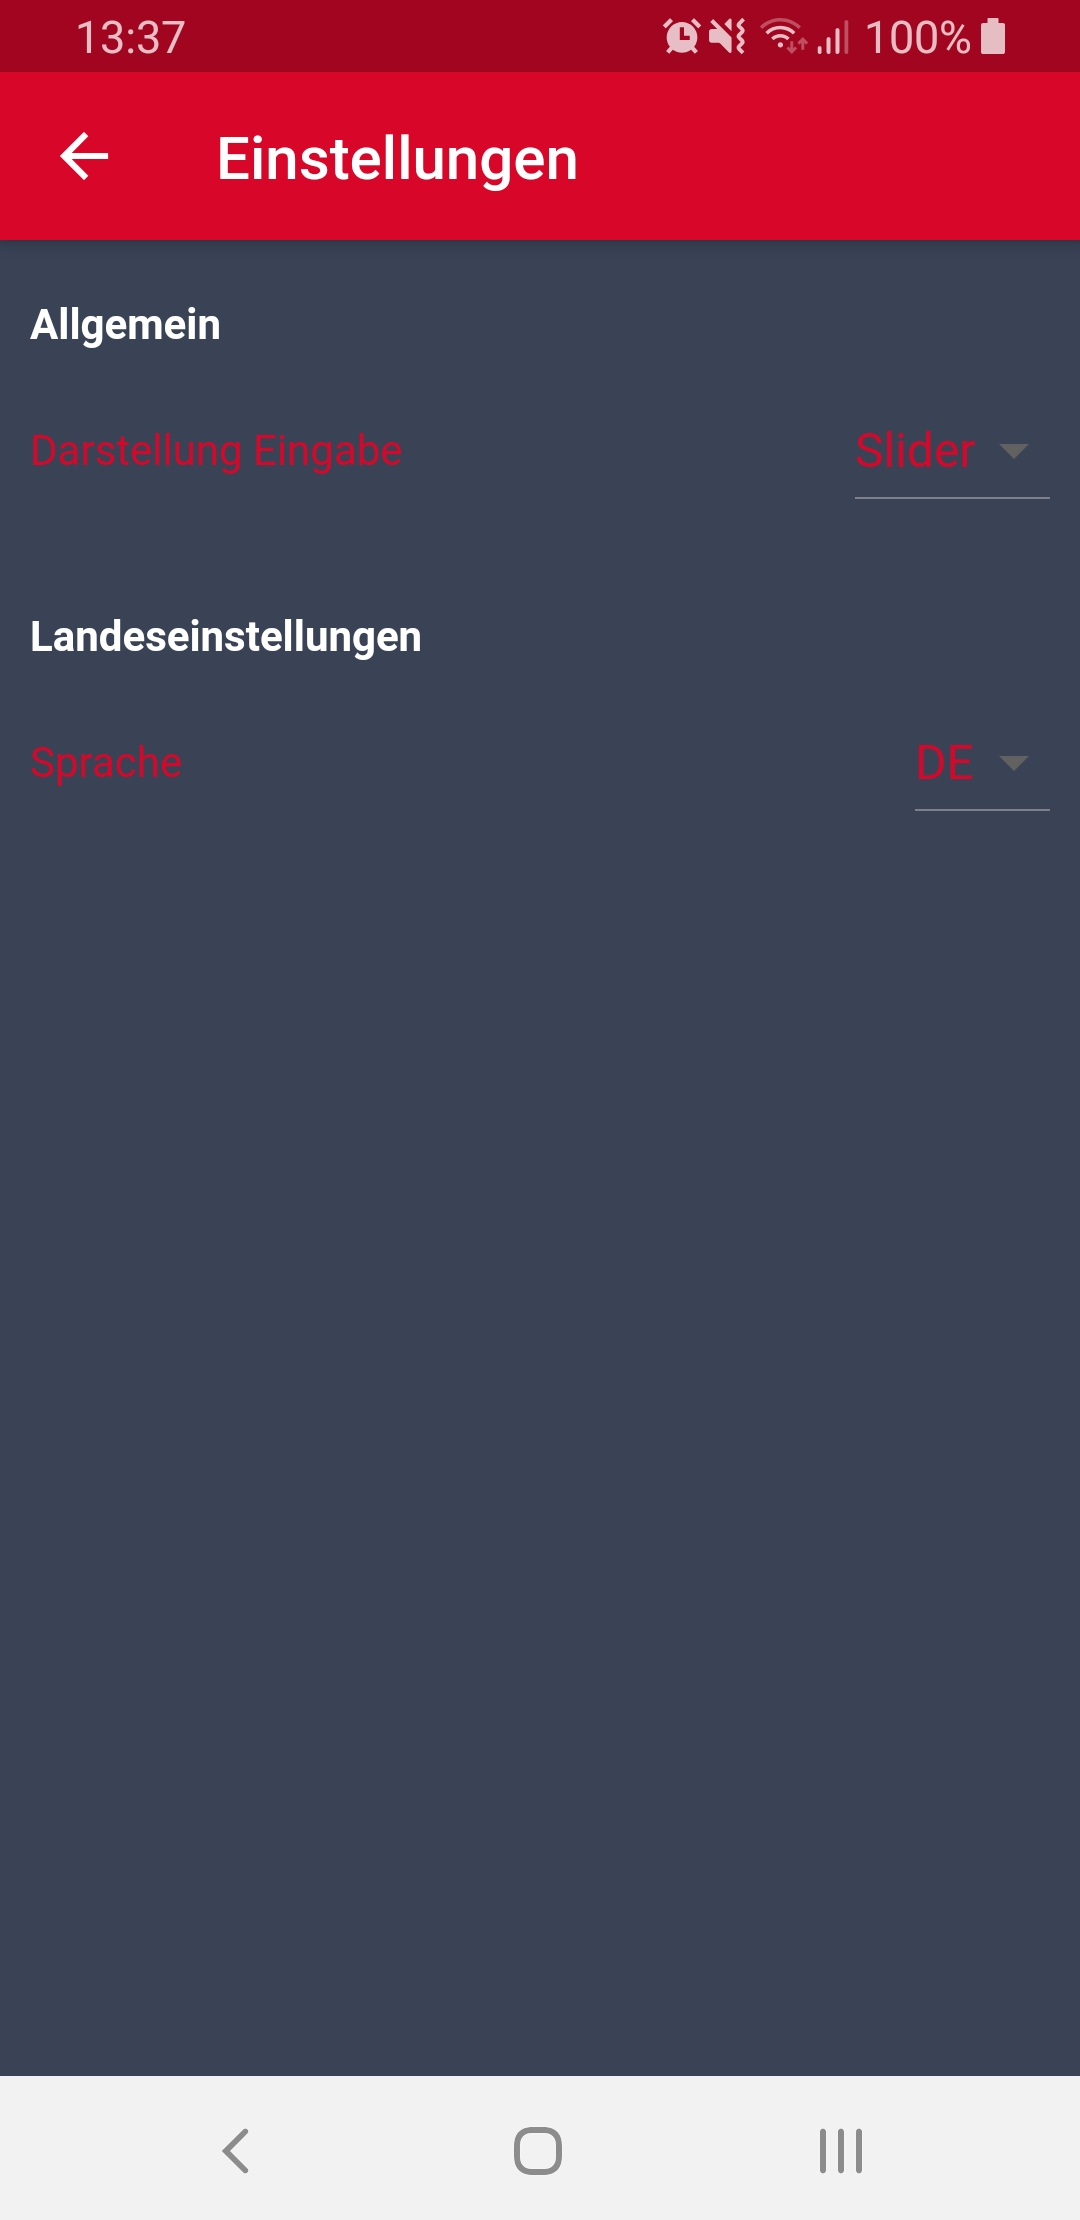
\includegraphics[width=1\textwidth]{../include/images/usertests/colorSettings/after}
		\end{subfigure}
		\caption{Links: Einstellungsseite vor dem Interview, rechts nach dem Interview}
		\label{img:colorSettings}
	\end{figure}
	
	Nach dem Feedback wurde die Einstellungsseite so angepasst, dass der Text der einzelnen Kategorien weiß und der Text der einzelnen Einstellungen dunkelrot ist. Diese Anpassung zog einige Anpassungen nach sich, weil zuvor das Flutter-Paket \textit{preferences} verwendet wurde. Dies lässt aber leider keine Konfiguration der Farben zu, sodass die komplette Einstellungsseite selbst programmiert werden musste. Der zu Grunde liegende |PrefService|, welcher auf die |SharedPreferences| zugreift, wird weiterhin verwendet. Das dynamische Setzen der Bedienungselemente wie die Auswahlliste und das automatische Speichern der neuen Werte musste nachprogrammiert werden. \cref{img:colorSettings} zeigt die Einstellungsseite vor und nach den Anpassungen
	
	
	\section{Benutzertest- und Interview 3}
	\label{sec:flinterview3}
	
	\paragraph{Wie ist der erste Eindruck?}
	
		Die App macht auf mich einen sehr guten Eindruck, es gibt keinen Punkt, der mich extrem gestört hat. Die Darstellung der einzelnen Daten ist sehr strukturiert, außerdem beschränkt sich die App auf das Wesentliche und ist nicht überladen. Dadurch war es sehr angenehm, sie zu benutzen. Insbesondere gefällt mir die Farbgebung sehr gut, das rot wirkt angenehm und auch die weiße Schrift in Kombination mit dem dunkelgrauen Hintergrund wirkt sehr stimmig.
	
	\paragraph{Was ist positiv aufgefallen?}
		
		Insgesamt hat mir die App sehr gut gefallen, sodass es keinen einzelnen Punkt gibt, den ich besonders hervorheben möchte. Die App als Ganzes wirkt in sich abgeschlossen und es gibt kein Element, welches in ihr ``fremd'' wirkt. Sie bietet einige Komfortfunktionen, beispielsweise das Einlesen der Simulationsdaten über einen zuvor generierten QR-Code, aber auch das Einlesen über die ID der Simulation ist sehr gut gelungen. Hat man die Daten als QR-Code zur Verfügung, wo ist die App komplett ohne Internet-Zugriff verwendbar, da alle Daten lokal auf dem Gerät gespeichert werden, auch dies ist ein positiver Aspekt.
	
	\paragraph{Was ist negativ aufgefallen?}
	
		Trotz aller zuvor erwähnten positiven Aspekte gibt es einen Punkt, den ich als störend empfunden habe: Befindet man sich auf der Seite, auf der die Simulationsergebnisse angezeigt werden, so ist es nicht möglich, das Profil zu wechseln, ohne den ganzen Weg ``zurückzugehen''. Dies ist insbesondere dann sehr nervig, wenn man mehrere Profile hat, zwischen denen man oft wechseln muss. Ich würde mir deshalb eine Funktion wünschen, durch die ich das Profil auch dann schnell wechseln kann, wenn ich mich auf der Seite mit den Simulationsergebnissen befinde.
	
	\paragraph{Ist die App intuitiv bedienbar?}
		
		Durch die Verwendung des \textit{Materialdesigns} passt sich die App nahtlos an bereits bestehende Apps an und wirkt nicht wie ein Fremdkörper. Dadurch fiel mir die Bedienung sehr leicht und ich habe keine weitere Hilfe benötigt. Außerdem werden bereits durch andere Apps etablierte Gesten wie das Wischen über ein Listenelement zum löschen verwendet, sodass sich die App auch in diesem Punkt gut eingliedert.
		
	\begin{figure}[H]
		\centering
		\begin{subfigure}[b]{0.45\textwidth}
			\centering
			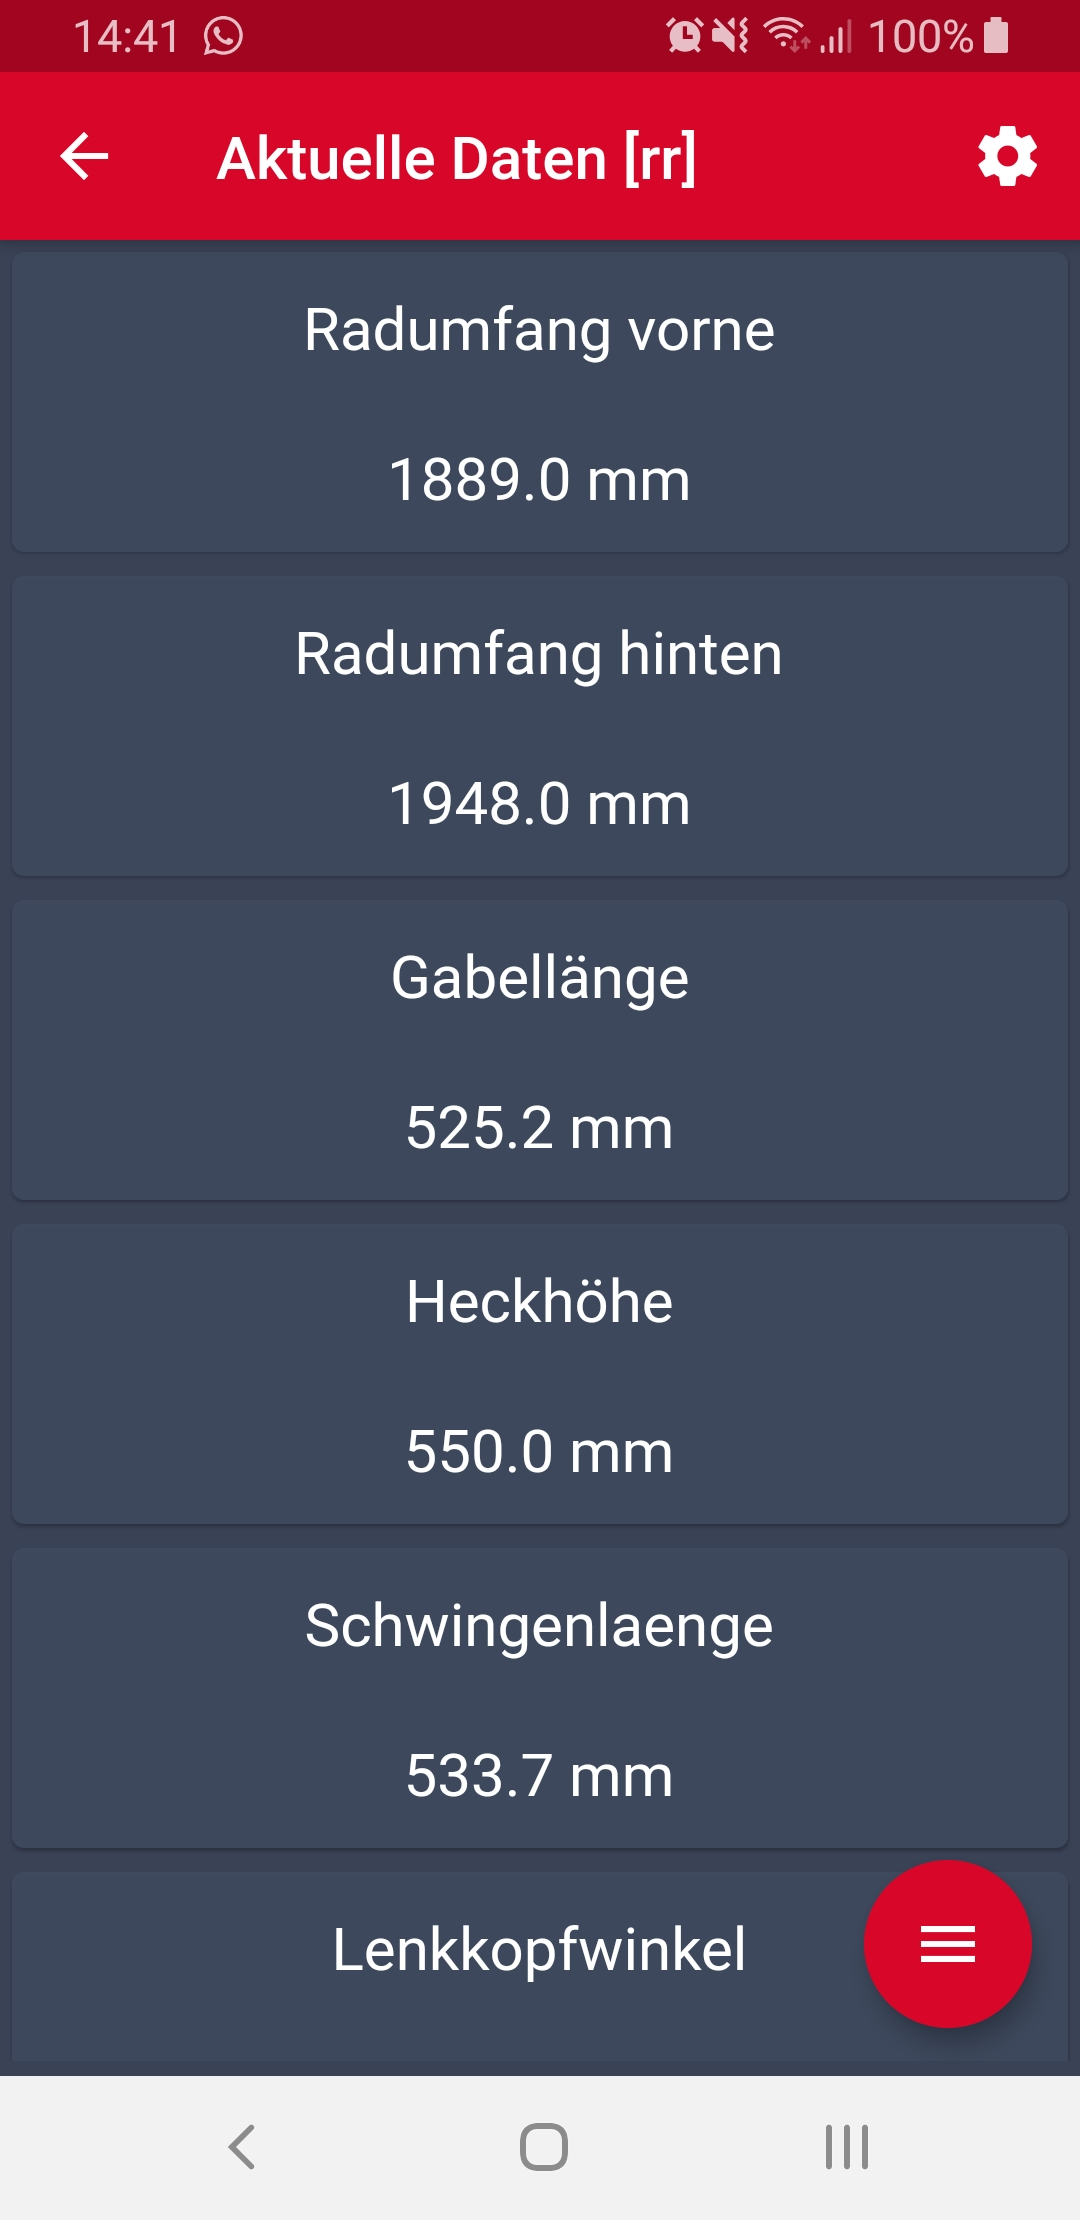
\includegraphics[width=1\textwidth]{../include/images/usertests/threepointmenu/before}
		\end{subfigure}
		\hfill
		\begin{subfigure}[b]{0.45\textwidth}
			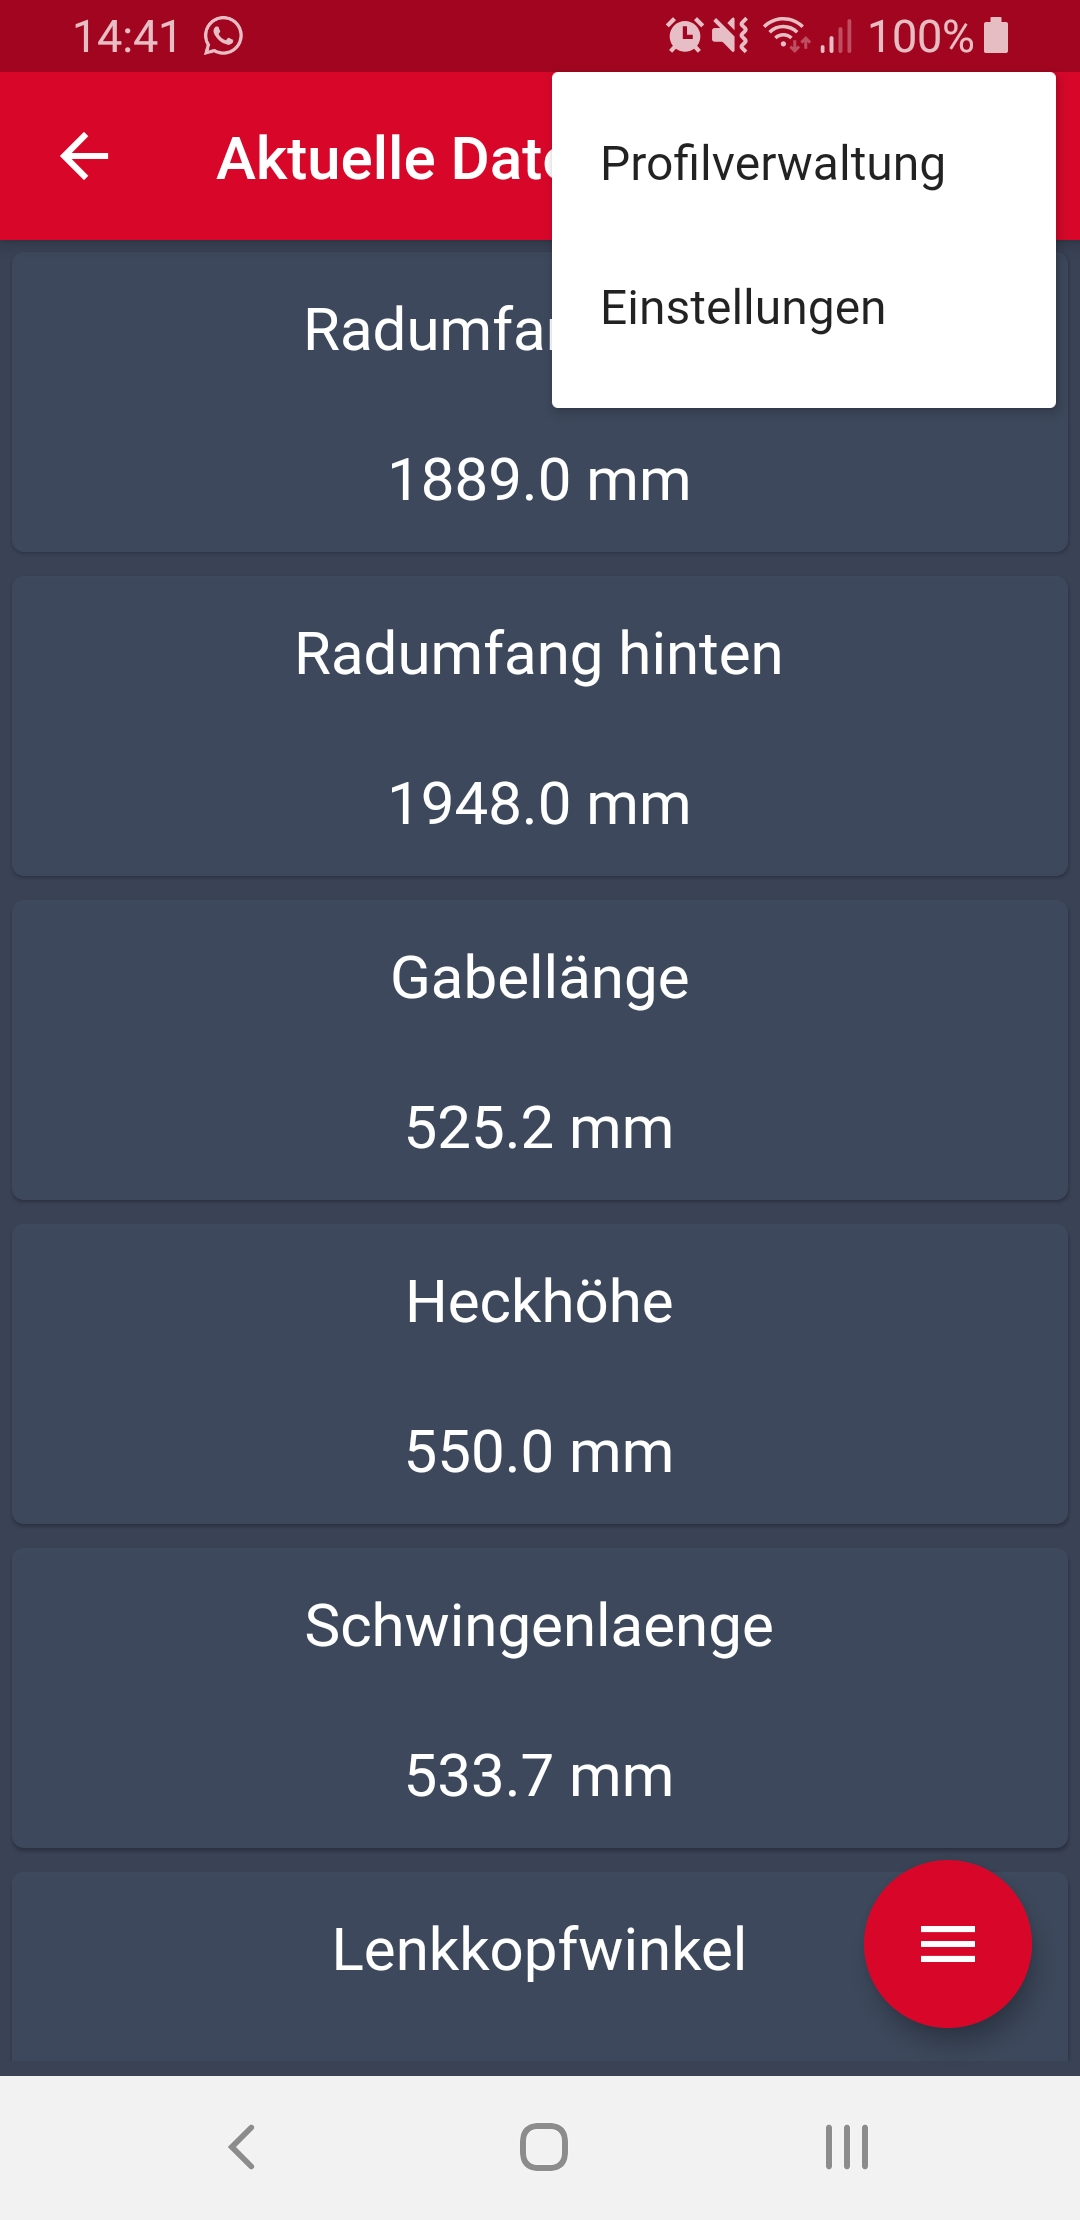
\includegraphics[width=1\textwidth]{../include/images/usertests/threepointmenu/after}
		\end{subfigure}
		\caption{Links: Übersichtsseite vor dem Interview, rechts nach dem Interview. Zu sehen ist das Drei-Punkt-Menü, was eine verbesserte Navigation ermöglicht.}
		\label{img:threepointmenu}
	\end{figure}

	Die Kritik des Probanden wurde zum Anlass genommen, die Navigation der App zu verändern: Befand man sich vorher auf der Seite, auf der die Ergebnisse der Simulation dargestellt werden, so musste man drei mal zurück gehen, um das Profil zu ändern. Nach der Anpassung ist dies nun über das Drei-Punkt-Menü möglich, die ist in ... zu sehen.